\documentclass{article}
\usepackage{graphicx} % 
\usepackage{amsmath}
\usepackage{booktabs}
\usepackage{graphicx}
\usepackage{multirow}
\usepackage{caption}
\usepackage{array}
\usepackage{float}
\usepackage{placeins}


\begin{document}

\title{Physics Collisions \\ Lab \#7 }
\author{Roxanne Rahimi, Maddie Jacobs, Ryan Mealia}
\date{Physics 4A - 62095 \\ Date Performed: October 14, 2024 \\ Due Date: October 19, 2024}



\maketitle
\centering
\begin{tabular}{|>{\raggedright\arraybackslash}m{4cm}|>{\centering\arraybackslash}m{4cm}|}
    \hline
    \textbf{RESEARCHER} & \textbf{SCALED GRADE} \\
    \hline
    Maddie Jacobs & \underline{\phantom{xxxxxxxx}} 10 \\
    \hline
\end{tabular}

\vspace{1cm}

\begin{tabular}{|>{\raggedright\arraybackslash}m{4cm}|>{\centering\arraybackslash}m{4cm}|}
    \hline
    \textbf{ANALYST} & \textbf{SCALED GRADE} \\
    \hline
    Roxanne Rahimi & \underline{\phantom{xxxxxxxx}} 10 \\
    \hline
\end{tabular}

\vspace{1cm}

\begin{tabular}{|>{\raggedright\arraybackslash}m{4cm}|>{\centering\arraybackslash}m{4cm}|}
    \hline
    \textbf{PRINCIPLE INVESTIGATOR} & \textbf{SCALED GRADE} \\
    \hline
    Ryan Mealia & \underline{\phantom{xxxxxxxx}} 10 \\
    \hline
\end{tabular}
\pagebreak
\section{Data Table}

\begin{table}[h!]
\centering
\caption*{\textbf{\underline{COLLISIONS EXPERIMENT}} \\ \textbf{DATA TABLE}}
\begin{tabular}{|>{\centering\arraybackslash}m{6cm}|>{\centering\arraybackslash}m{6cm}|}
\hline
\textbf{LEFT CART MASS} & \textbf{} \\ 
\textbf{$m_A \pm \delta m_A$} & \textbf{$0.2731 \pm 0.0001$} \\
\text {kg} & \multirow{2}{*}{} \\
(Blue) & \\ \hline
\textbf{RIGHT CART MASS} & \textbf{} \\
\textbf{$m_B \pm \delta m_B$} & \textbf{$0.2747 \pm 0.0001$} \\
\text {kg} & \multirow{2}{*}{} \\
(Red) & \\ \hline
\end{tabular}
\end{table}


\begin{table}[H]
\centering
\begin{tabular}{|c|c|c|}
\hline
\textbf{COLLISION SCENARIO} & \multicolumn{2}{c|}{\textbf{INITIAL HORIZONTAL VELOCITY}} \\ 
\hline
 & \textbf{LEFT CART} & \textbf{RIGHT CART} \\
 & $V_{A0X} \pm \delta V_{A0X}$ & $V_{B0X} \pm \delta V_{B0X}$ \\
 & (m/s) & (m/s) \\
\hline
First & $0.325 \pm 0.0095$ & $-9.13 \cdot 10^{-5} \pm 3.7 \cdot 10^{-5}$ \\
\hline
Second & $0.357 \pm 0.0041$ & $-0.120 \pm 0.0017$ \\
\hline
Third & $0.319 \pm 7.7 \cdot 10^{-4}$ & $0.373 \pm 0.0013$ \\
\hline
\end{tabular}
\caption{Initial Horizontal Velocity}
\label{tab:initial_velocity}
\end{table}

% Second Table

\begin{table}[H]
\centering
\begin{tabular}{|c|c|c|}
\hline
\textbf{COLLISION SCENARIO} & \multicolumn{2}{c|}{\textbf{FINAL HORIZONTAL VELOCITY}} \\ 
\hline
 & \textbf{LEFT CART} & \textbf{RIGHT CART} \\
 & $V_{AX} \pm \delta V_{AX}$ & $V_{BX} \pm \delta V_{BX}$ \\
 & (m/s) & (m/s) \\
\hline
First & $1.23 \cdot 10^{-5} \pm 4.7 \cdot 10^{-5}$ & $-0.356 \pm 9 \cdot 10^{-4}$ \\
\hline
Second & $0.101 \pm 3.3 \cdot 10^{-4}$ & $-0.353 \pm 7.2 \cdot 10^{-4}$ \\
\hline
Third & $-0.319 \pm 0.0016$ & $-0.297 \pm 3.8 \cdot 10^{-4}$ \\
\hline
\end{tabular}
\caption{Final Horizontal Velocity}
\label{tab:final_velocity}
\end{table}

\section{Graphs}
\begin{figure}[H]
    \centering
    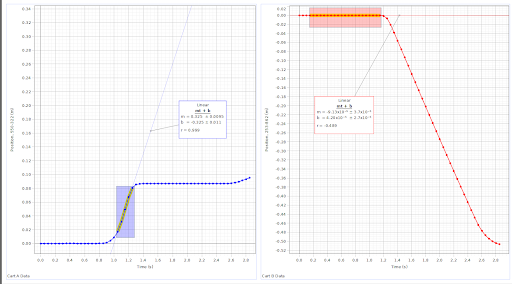
\includegraphics[width=0.75\linewidth]{first scenario initial .png}
    \caption{First Scenario Initial}
    \label{fig:fsi}
\end{figure}
\begin{figure}[H]
    \centering
    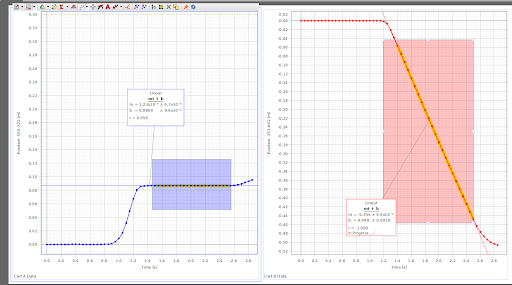
\includegraphics[width=0.75\linewidth]{first scenario final.png}
    \caption{First Scenario Final}
    \label{fig:fsf}
\end{figure}
\begin{figure}[H]
    \centering
    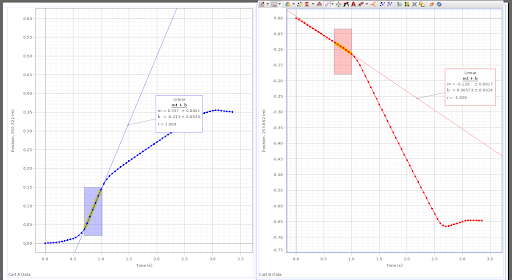
\includegraphics[width=0.75\linewidth]{second scenario initial.png}
    \caption{Second Scenario Initial}
    \label{fig:ssi}
\end{figure}
\begin{figure}[H]
    \centering
    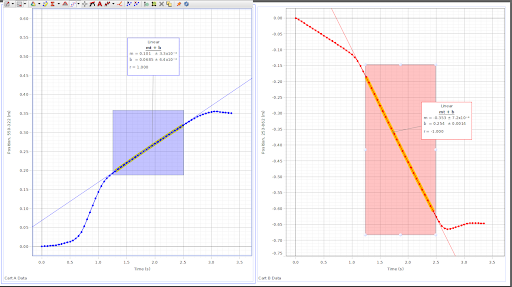
\includegraphics[width=0.75\linewidth]{second scenario final.png}
    \caption{Second Scenario Final}
    \label{fig:ssf}
\end{figure}
\begin{figure}[H]
    \centering
    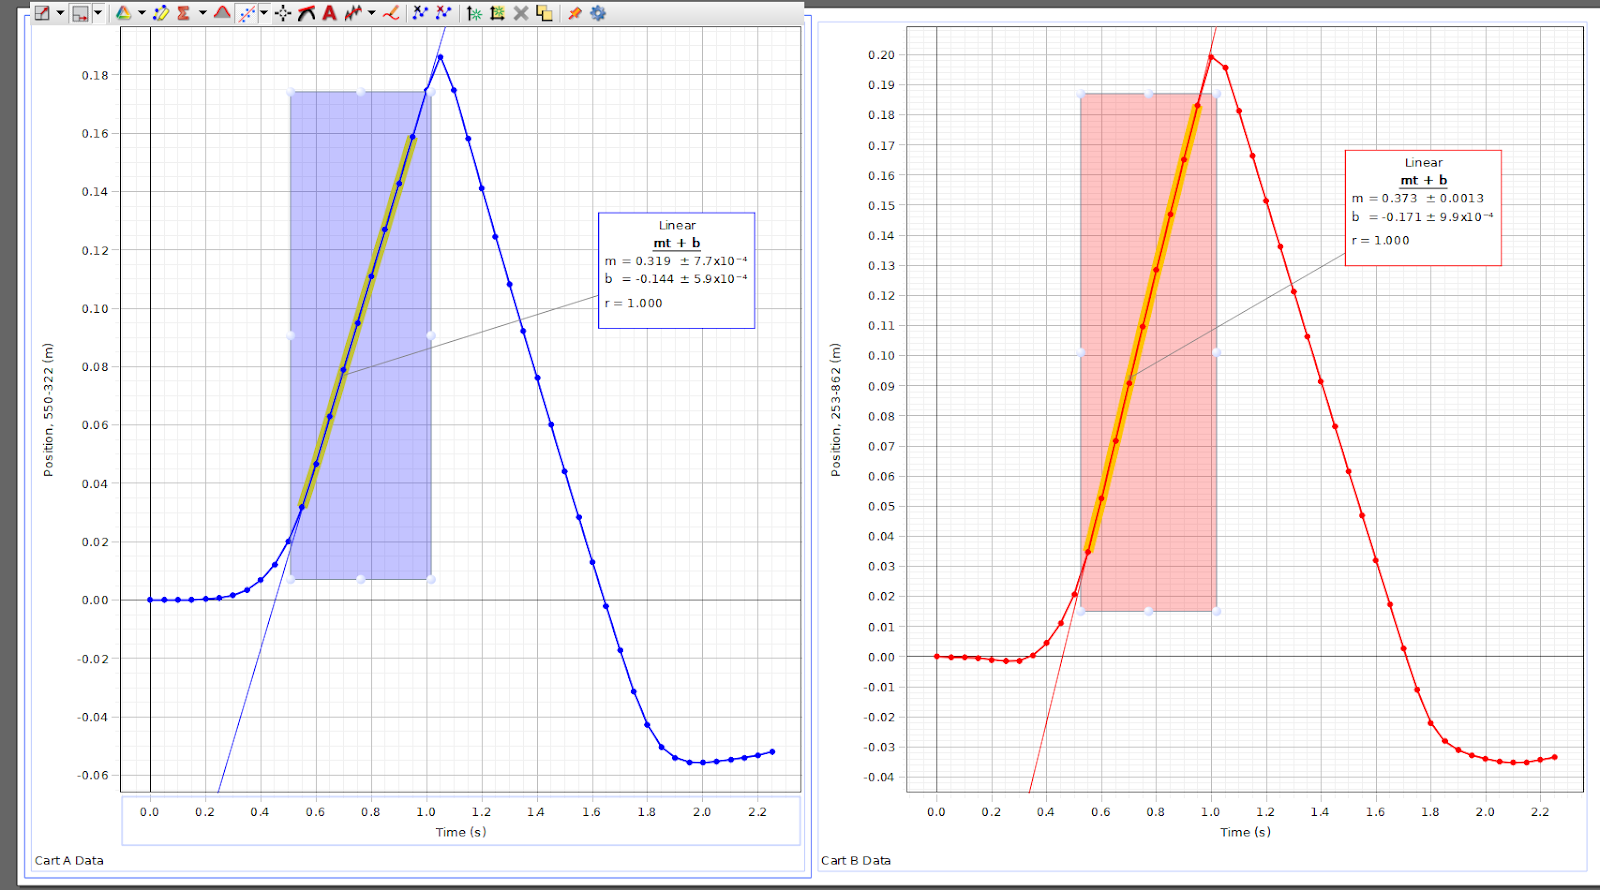
\includegraphics[width=0.75\linewidth]{third scenario initial.png}
    \caption{Third Scenario Initial}
    \label{fig:tsi}
\end{figure}
\begin{figure}[H]
    \centering
    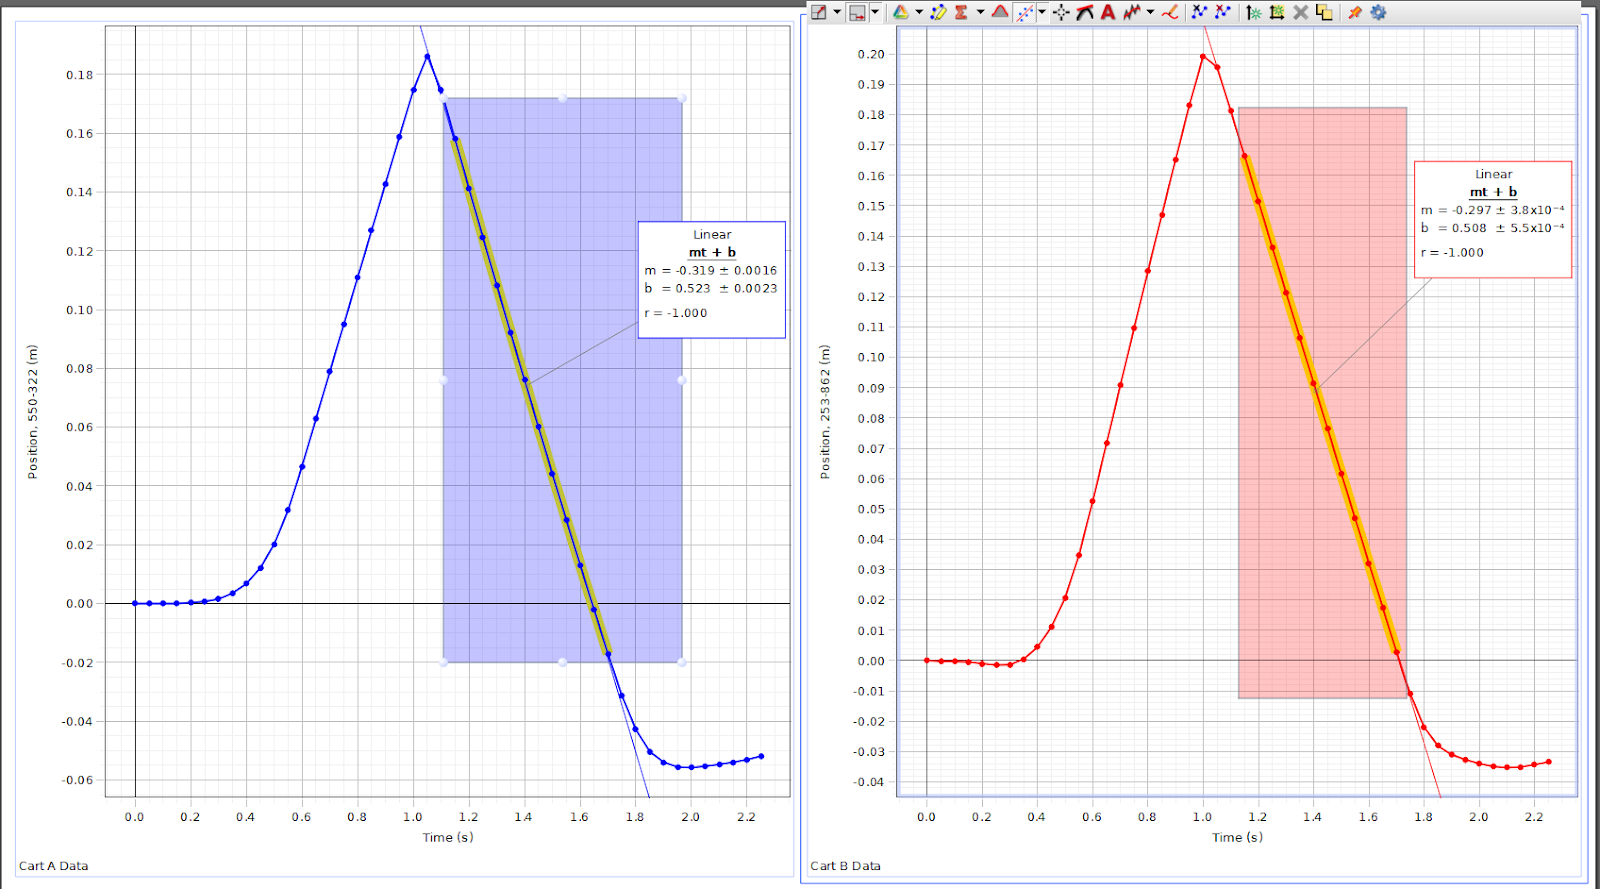
\includegraphics[width=0.75\linewidth]{third scenario final.png}
    \caption{Third Scenario Final}
    \label{fig:tsf}
\end{figure}

\section{Calculations}
\subsection{Initial Mechanical Energy}
\subsubsection{First Scenario}
$E_{\text {mec, first}}=(\frac {1}{2})(0.2731 {kg})(0.325 \frac {m}{s^2})^2 +(\frac {1}{2})(0.2747 {kg})(-9.13 \times 10^{-5} {\frac {m}{s^2})}^2 $
\newline 
$E_{\text {mec, first}} = 0.0144 \text { J}$
\subsubsection{Second scenario}
$E_{\text {mec, second}}=(\frac {1}{2})(0.2731 {kg})(0.357 \frac {m}{s^2})^2 +(\frac {1}{2})(0.2747 {kg})(-0.120 {\frac {m}{s^2})}^2 $
\newline
$E_{\text {mec, second}} = 0.0194 \text { J}$
\subsubsection{Third scenario}
$E_{\text {mec, third}}=(\frac {1}{2})(0.2731 {kg})(0.319 \frac {m}{s^2})^2 +(\frac {1}{2})(0.2747 {kg})(0.373 {\frac {m}{s^2})}^2 $
\newline
$E_{\text {mec, third}} = 0.0330 \text { J}$


\subsection{Initial Mechanical Energy Uncertainty}
\subsubsection{First scenario}
$\delta E_{\text {mec, first  cart}} = \sqrt{((0.2731)(0.325))^2(0.0095)+((\frac {1}{2})(0.325)^2)^2(0.0001)^2}$
\newline
$\delta E_{\text {mec, first  cart}} = 0.00084 $
\newline

\subsubsection{Second scenario}
$\delta E_{\text {mec, second  cart}} = \sqrt{((0.2731)(0.357))^2(0.0041)+((\frac {1}{2})(0.357)^2)^2(0.0001)^2}$
\newline
$\delta E_{\text {mec, second  cart}} = 0.00040 $
\newline 

\subsubsection{Third scenario}
$\delta E_{\text {mec, third  cart}} = \sqrt{((0.2731)(0.319))^2(7.7 \times 10^{-4})+((\frac {1}{2})(0.319)^2)^2(0.0001)^2}$
\newline
$\delta E_{\text {mec, third  cart}} = 6.73 \times 10^{-5} $
\subsection{Final Mechanical Energy}
\subsubsection{first scenario}
$E_{\text {mec, first cart}} = (\frac {1}{2})(0.2731)(1.23 \times 10^{-5})^2+(\frac {1}{2})(0.2731)(-0.356)^2$
\newline
$E_{\text {mec, first cart}} = 0.0173 \text { J}$
\subsubsection{second scenario}
$E_{\text {mec, second cart}} = (\frac {1}{2})(0.2731)(0.101)^2+(\frac {1}{2})(0.2731)(-0.353)^2$
\newline
$E_{\text {mec, second cart}} = 0.0184 \text { J}$
\subsubsection{third scenario}
$E_{\text {mec, third cart}} = (\frac {1}{2})(0.2731)(-0.319)^2+(\frac {1}{2})(0.2731)(-0.297)^2$
\newline
$E_{\text {mec, third cart}} = 0.0259 \text { J}$
\subsection{Final Mechanical Energy Uncertainty}
\subsubsection{First Scenario}

\[
E_{\text{first cart}} = \sqrt{
    \left( \frac{1}{2} \left( 1.23 \times 10^{-5} \right)^2 + \frac{1}{2} \left( 0.2747 \right) \left( -0.356 \right)^2 \right)^2 \left( 0.0001 \right)^2 +
}
\]
\[
\left[
    \frac{1}{2} \left( 0.2731 \right) \left( 1.23 \times 10^{-5} \right)^2 + \frac{1}{2} \left( -0.356 \right)^2
\right]^2 \left( 0.0001 \right)^2 +
\]
\[
\left[
    \left( 0.2731 \right) \left( 1.23 \times 10^{-5} \right) + \frac{1}{2} \left( 0.2747 \right) \left( -0.356 \right)^2
\right]^2 \left( 4.7 \times 10^{-5} \right)^2 +
\]
\[
\left[
    \frac{1}{2} \left( 0.2731 \right) \left( 1.23 \times 10^{-5} \right)^2 + \left( 0.2747 \right) \left( -0.356 \right)
\right]^2 \left( 9 \times 10^{-4} \right)^2
\]

$E_{\text{first cart}} = 8.83 \times 10^{-5}$

\subsubsection{Second Scenario}

\[
E_{\text{second cart}} = \sqrt{
    \left( \frac{1}{2} \left( 0.101 \right)^2 + \frac{1}{2} \left( 0.2747 \right) \left( -0.353 \right)^2 \right)^2 \left( 0.0001 \right)^2 +
}
\]
\[
\left[
    \frac{1}{2} \left( 0.2731 \right) \left( 0.101 \right)^2 + \frac{1}{2} \left( -0.353 \right)^2
\right]^2 \left( 0.0001 \right)^2 +
\]
\[
\left[
    \left( 0.2731 \right) \left( 0.101 \right) + \frac{1}{2} \left( 0.2747 \right) \left( -0.353 \right)^2
\right]^2 \left( 3.3 \times 10^{-4} \right)^2 +
\]
\[
\left[
    \frac{1}{2} \left( 0.2731 \right) \left( 0.101 \right)^2 + \left( 0.2747 \right) \left( -0.353 \right)
\right]^2 \left( 7.2 \times 10^{-4} \right)^2
\]

$E_{\text{second cart}} = 7.07 \times 10^{-5}$



\subsubsection{Third Scenario}

\[
E_{\text{third cart}} = \sqrt{
    \left( \frac{1}{2} \left( -0.319 \right)^2 + \frac{1}{2} \left( 0.2747 \right) \left( -0.297 \right)^2 \right)^2 \left( 0.0001 \right)^2 +
}
\]
\[
\left[
    \frac{1}{2} \left( 0.2731 \right) \left( -0.319 \right)^2 + \frac{1}{2} \left( -0.297 \right)^2
\right]^2 \left( 0.0001 \right)^2 +
\]
\[
\left[
    \left( 0.2731 \right) \left( -0.319 \right) + \frac{1}{2} \left( 0.2747 \right) \left( -0.297 \right)^2
\right]^2 \left( 0.0016 \right)^2 +
\]
\[
\left[
    \frac{1}{2} \left( 0.2731 \right) \left( -0.319 \right)^2 + \left( 0.2747 \right) \left( -0.297 \right)
\right]^2 \left( 3.8 \times 10^{-4} \right)^2
\]

$E_{\text{third cart}} = 1.23 \times 10^{-4}$
\subsection{Percent Differences}
$PD_{\text {first}}=\frac{|0.0144-0.0173|}{\frac{0.0144+0.0173}{2}}\times 100 $
\newline
$PD_{\text {first}}=18.30\%$
\newline
\newline
$PD_{\text {second}}=\frac{|0.0194-0.0184|}{\frac{0.0194+0.0184}{2}}\times 100 $
\newline
$PD_{\text {second}}= 5.29 \%$
\newline 
\newline
$PD_{\text {third}}=\frac{|0.033-0.0259|}{\frac{0.033+0.0259}{2}}\times 100 $
\newline
$PD_{\text {third}}=24.11 \%$
\section{Table Of Results}

\begin{table}[h!]
\centering
\caption*{\textbf{TABLE OF RESULTS}}
\begin{tabular}{|c|c|c|}
\hline
\multirow{2}{*}{\textbf{COLLISION SCENARIO}} & \multicolumn{2}{c|}{\textbf{MECHANICAL ENERGY}} \\ \cline{2-3} 
 & \textbf{INITIAL $E_{\text{mec,0}} \pm \delta E_{\text{mec,0}}$ (J)} & \textbf{FINAL $E_{\text{mec}} \pm \delta E_{\text{mec}}$ (J)} \\ \hline
\textbf{First} & $0.0144 \pm 0.00084$ & $0.0173 \pm 8.83 \times 10^{-5}$ \\ \hline
\textbf{Second} & $0.0194 \pm 0.00040$ & $0.0184 \pm 7.07 \times 10^{-5}$ \\ \hline
\textbf{Third} & $0.0330 \pm 6.73 \times 10^{-5}$ & $0.0259 \pm 1.23 \times 10^{-4}$ \\ \hline
\end{tabular}
\end{table}

\begin{table}[h!]
\centering
\begin{tabular}{|c|c|}
\hline
\textbf{COLLISION SCENARIO} & \textbf{MECHANICAL ENERGY PERCENT DIFFERENCE $PD$ (\%)} \\ \hline
\textbf{First} & 18.30\% \\ \hline
\textbf{Second} & 5.29\% \\ \hline
\textbf{Third} & 24.11\% \\ \hline
\end{tabular}
\end{table}
\section{Questions}


\parindent
\textbf{Overall, were the initial mechanical energies precise or imprecise? Justify your answer.} \vspace{0.25cm}
\par
\newline
The precision of the initial mechanical energies are calculated by analyzing the uncertainties in the values. The uncertainty for the first scenario was 0.00084. For the second scenario it was 0.00040 and for the last scenario it was 0.0000673. All of these are extremely small uncertainties. 
Precision refers to the consistency of measurements. An uncertainty quantifies the possible range for values within the true measured amount. Therefore, the super small uncertainties show high confidence in the measurement. It means we are more confident that the true value is close to the measured value, within a small range - which is exactlty what high precision means. \vspace{0.5cm}



\textbf{Overall, was the final mechanical energies precise or imprecise? Justify your answer.}\vspace{0.25cm}
\newline
Again, the final mechanical energies also have extremely small uncertainties in relation to the measured mechanical energies. For example, for the first scenario it is $8.83 \times 10^{-5}$. For the second scenario it is $1.23 \times 10^{-4}$. For the third scenario it is $1.23 \times 10^{-4}$. These are all extremely small meaning that there is such a small uncertainty if the measured value is precise. As explained above, if the calculated uncertainty were to be larger that means that the maeasurement could vary widely, which means there is less confidence in how close the measured value is to the true value. A large uncertainty would mean that there is a larger range of possible values - meaning that the values are not close to each other and therefore imprecise. \vspace{0.5cm}

\textbf{Overall, was mechanical energy conserved? Justify your answer.}\vspace{0.25cm}
\newline
To determine whether mechanical energy was conserved, we can compare the initial and final mechanical energies for each scenario. The first scenario had a percent difference of 18.30\%. The second scenario had a percent difference of 5.20\%. The third scenario had a percent difference of 24.11\%. These are relatively high percentages with the exception of the second scenario. But, the mechanical energy was not really conserved for either of these scenarios. The second scenario's small percent difference suggests that it conserved most mechanical energy. But, the first and third scenario show relatively large losses. These were likely due to friction, air resistance, and imperfections in elastic collisions. Theoretically, mechanical energy should have been conserved in this experiment for the collisions to be perfectly elastic. Ideally, no kinetic energy should be lost, and mechanical energy should remain constant. But, there was definitely friction between the carts, air resistance, and the collisions were probably not completely elastic. \vspace{0.5cm}   

\textbf{Identify the independent variable(s) for this experiment.
Be specific and use proper vocabulary.}\vspace{0.25cm}
\newline
The independent variables are variables that occur individually and do not rely on anything else for their results. The initial velocities of the carts are independent. The varying initial velocities within each scenario caused different outcomes. The outcomes relied on these such independent variables. But, these independent variables don't occur on the basis of something else occuring \vspace{0.5cm}


\textbf{Identify the fixed variable(s) for this experiment.
Be specific and use proper vocabulary.}\vspace{0.25cm}
\newline
Fixed variables are those that are defined at the start, before the experiment, and remain unchanged throughout the different scenarios.
The fixed variables in the experiment are the masses of each of the carts. These masses were recorded once before any of the trials and remained constant throughout the experiment. 
Experimental conditions, such as the track being level or the environment we did the experiment in remained constant. This is important because friction remained relatively constant since these things were unchanged.\vspace{0.5cm}


\textbf{Identify the dependent variable(s) for this experiment.
Be specific and use proper vocabulary.} \vspace{0.25cm}
\newline
The dependent variables are things that rely on the conditions and on the independent variable to be specific. Therefore, the dependent variable was the final velocities of the carts since it in part relied on the independent variable, which were the independent variables. The calculated final mechanical energies from the graphs shown by the PASCO system depended on the initial velocities of the cart as well. \vspace{0.5cm}
\newline
\textbf{Conclusion} \vspace{0.25cm}
\newline
In conclusion, this experiment aimed to demonstrate the conservation of mechanical energy with 2 carts colliding in different ways on a track. The results show that the mechanical energy was not fully conserved during any of the collisions. We had larger percent differences between the initial and final mechanical energies. These losses were probably a result of friction, air resistance, and the fact that these collisions were probably not 100\% elastic to begin with. Most things in every-day life are not perfectly elastic. However, we had a relatively high precision within our data. To improve this lab, we could reduce the friction on the track by using a low friction track. The friction between the carts and the tracks probably accounted for at least some of the mechanical energy being not fully conserved. Additionally, we could conduct the experiment in a vacuum chamber to minimize air resistance. We could also do multiple trials to reduce uncertainty if random errors occur. 
\newline 
Also, it is important to note that some of our initial data had abnormal signs but it doesn't matter much since these values were squared when calculating different things. We just oriented the cars differently. 

\end{document}


